\documentclass[11pt]{article}
\usepackage{amssymb}
\usepackage{amsthm}
\usepackage{enumitem}
\usepackage{physics,amsmath}
\usepackage{bm}
\usepackage{adjustbox}
\usepackage{mathrsfs}
\usepackage{graphicx}
\usepackage{siunitx}
\usepackage[mathscr]{euscript}


\title{\textbf{Solved selected problems of General Relativity - Thomas A. Moore}}
\author{Franco Zacco}
\date{}

\addtolength{\topmargin}{-3cm}
\addtolength{\textheight}{3cm}

\newcommand{\hatr}{\bm{\hat{r}}}
\newcommand{\hatn}{\bm{\hat{n}}}
\newcommand{\hatx}{\bm{\hat{x}}}
\newcommand{\haty}{\bm{\hat{y}}}
\newcommand{\hatz}{\bm{\hat{z}}}
\newcommand{\hatth}{\bm{\hat{\theta}}}
\newcommand{\hatphi}{\bm{\hat{\phi}}}
\newcommand{\hatrho}{\bm{\hat{\rho}}}
\newcommand{\er}{\bm{e}_r}
\newcommand{\etht}{\bm{e}_\theta}
\newcommand{\sci}[1]{\times 10^{#1}}

\theoremstyle{definition}
\newtheorem*{solution*}{Solution}
\renewcommand*{\proofname}{Solution}

\begin{document}
\maketitle
\thispagestyle{empty}

\section*{Chapter 14 - Event Horizon}

\begin{proof}{\textbf{BOX 14.1} - Exercise 14.1.1.}\\
Let
\begin{align*}
    u = \sqrt{1 - \frac{2GM}{r}}
\end{align*}
Then
\begin{align*}
    u^2 &= 1 - \frac{2GM}{r}\\
    \frac{2GM}{r} &= 1 - u^2\\
    r &= \frac{2GM}{1 - u^2}
\end{align*}
\end{proof}
\begin{proof}{\textbf{BOX 14.1} - Exercise 14.1.2.}\\
Let
\begin{align*}
    r &= \frac{2GM}{1 - u^2}
\end{align*}
Then
\begin{align*}
    \dv{r}{u} &= \frac{4GMu}{(1 - u^2)^2}\quad\text{hence}\quad
    dr = \frac{4GMu}{(1 - u^2)^2}~du
\end{align*}
Replacing in (14.7) we have that
\begin{align*}
    \Delta s = \int \frac{4GM u du}{u (1 - u^2)^2} = 4GM \int \frac{du}{(1 - u^2)^2}
\end{align*}
Finally, since we want to integrate between $r = 2GM$ and $r = R$ then $u$ at
$2GM$ is $0$ so we write 
\begin{align*}
    \Delta s = 4GM \int_0^{u(R)} \frac{du}{(1 - u^2)^2}
\end{align*}
\end{proof}
\begin{proof}{\textbf{BOX 14.1} - Exercise 14.1.3.}\\
Knowing that
\begin{align*}
    \int \frac{du}{(1 - u^2)^2} = \frac{u}{2(1 - u^2)}
    + \frac{1}{4}\log\bigg|\frac{1 + u}{1 - u}\bigg|
\end{align*}
and that
\begin{align*}
    \tanh^{-1} u = \frac{1}{2}\log\bigg|\frac{1 + u}{1 - u}\bigg|
\end{align*}
We can solve $\Delta s$ equation as follows
\begin{align*}
    \Delta s &= 4GM \int_0^{u(R)} \frac{du}{(1 - u^2)^2}\\
    &= 4GM \bigg[\frac{u}{2(1 - u^2)} + \frac{\tanh^{-1} u}{2}\bigg]_0^{u(R)}\\
    &= 4GM \bigg[\frac{u(R)}{2(1 - u(R)^2)} + \frac{\tanh^{-1} u(R)}{2} - 0\bigg]
\end{align*}
Finally, we replace back $u(R) = \sqrt{1 - 2GM/R}$
\begin{align*}
    \Delta s 
    &= 4GM \bigg[\frac{\sqrt{1 - 2GM/R}}{4GM/R}
    + \frac{\tanh^{-1} \sqrt{1 - 2GM/R}}{2}\bigg]\\
    &= R\sqrt{1 - 2GM/R} + 2GM\tanh^{-1} \sqrt{1 - 2GM/R}
\end{align*}
\end{proof}
\begin{proof}{\textbf{BOX 14.1} - Exercise 14.1.4.}\\
Let now $R = 3GM$ then the physical distance from $r=2GM$ to $R = 3GM$ is
\begin{align*}
    \Delta s 
    &= 3GM\sqrt{1 - 2/3} + 2GM\tanh^{-1} \sqrt{1 - 2/3}\\
    &= 3GM\sqrt{1/3} + 2GM\tanh^{-1} \sqrt{1/3}\\
    &= 1.7320~GM + 1.3169~GM\\
    &= 3.048~GM
\end{align*}

\end{proof}

\cleardoublepage
\begin{proof}{\textbf{BOX 14.2} - Exercise 14.2.1.}\\
Let
\begin{align*}
    \Delta\tau
    &= 2\sqrt{\frac{R}{2GM}}\int_0^{u_0} \frac{u^2 du}{\sqrt{u_0^2 - u^2}}
\end{align*}
Then
\begin{align*}
    \Delta\tau
    &= \sqrt{\frac{R}{2GM}}\bigg[
        u_0^2\arctan(\frac{u}{\sqrt{u_0^2 - u^2}}) - u\sqrt{u_0^2 - u^2}
    \bigg]_0^{u_0}\\
    &= \sqrt{\frac{R}{2GM}}\bigg[u_0^2\frac{\pi}{2} - 0\bigg]\\
    &= \frac{\pi}{2}R\sqrt{\frac{R}{2GM}}\\
    &= \frac{\pi}{2}\sqrt{\frac{R^3}{2GM}}
\end{align*}
\end{proof}
\begin{proof}{\textbf{BOX 14.3} - Exercise 14.3.1.}\\
Let 
\begin{align*}
    \Delta\tau &= \int_0^{2GM} \frac{r^{1/2} dr}{\sqrt{2GM - r}}
\end{align*}
Then letting $u = \sqrt{r}$ we have that
\begin{align*}
    \Delta\tau &= 2\int_0^{\sqrt{2GM}} \frac{u^2 du}{\sqrt{2GM - u^2}}
\end{align*}
Hence
\begin{align*}
    \Delta\tau
    &= \bigg[
        2GM\arctan(\frac{u}{\sqrt{2GM - u^2}}) - u\sqrt{2GM - u^2}
    \bigg]_0^{\sqrt{2GM}}\\
    &= \bigg[2GM\frac{\pi}{2} - 0\bigg]\\
    &=\pi GM
\end{align*}
\end{proof}

\cleardoublepage
\begin{proof}{\textbf{P14.1}}
From BOX 14.2 we know that the proper time (measured by our own watch) we have
to live until we reach $r = 0$ when we started from a radially inward fall
from $r = R$ is 
\begin{align*}
    \Delta\tau &= \frac{\pi}{2}\sqrt{\frac{R^3}{2GM}}
\end{align*}
In our current case $R = 10GM$ hence
\begin{align*}
    \Delta\tau &= \frac{\pi}{2}\sqrt{\frac{(10GM)^3}{2GM}}\\
    &= 35.124 GM\\
    &= 35.124\cdot 1477 \cdot 10^6~m\\
    &= 51878256788.735~m\\
    &= 173.042~s
\end{align*}
Where we used that $299800~km = 1~s$.
\end{proof}

\cleardoublepage
\begin{proof}{\textbf{P14.2}}
\begin{itemize}
\item [\textbf{a.}] The time the clock registers between its launch at
$r = 16GM$ and when it comes to rest at $r = 32GM$ is the same time it
registers between falling from rest from $32GM$ to $r = 16GM$ hence,
we can compute this time using the equation from BOX 14.2 as follows
\begin{align*}
    \Delta \tau &= \sqrt{\frac{32GM}{2GM}}\bigg[
        32GM\arctan(\frac{u}{\sqrt{32GM - u^2}}) - u\sqrt{32GM - u^2}
    \bigg]_{\sqrt{16GM}}^{\sqrt{32GM}}\\
    &= 4\bigg[ 16\pi GM -  8\pi GM + 16GM \bigg]\\
    &= 164.53 \cdot 1477 \cdot 10^6\\
    &= 243010810000.0~m = 810.57~s
\end{align*}
\item [\textbf{b.}] In the same way, the time the clock registers between being
at rest at $r = 32GM$ and falling to $r = 2GM$ (the event horizon) is
\begin{align*}
    \Delta \tau &= \sqrt{\frac{32GM}{2GM}}\bigg[
        32GM\arctan(\frac{u}{\sqrt{32GM - u^2}}) - u\sqrt{32GM - u^2}
    \bigg]_{\sqrt{2GM}}^{\sqrt{32GM}}\\
    &= 4\bigg[ 16\pi GM - 8.085GM + 7.746GM \bigg]\\
    &= 199.705 \cdot 1477 \cdot 10^6\\
    &= 294964285000.0~m = 983.87~s
\end{align*}
\item [\textbf{c.}] Finally, to compute the time the clock registers between
crossing the event horizon and its destruction at the origin, we need to compute
the time it registers from falling at rest from $r=32GM$ to $r=0$ and then
subtract the time we computed in part \textbf{b.}
\begin{align*}
    \Delta \tau &= \sqrt{\frac{32GM}{2GM}}\bigg[
        32GM\arctan(\frac{u}{\sqrt{32GM - u^2}}) - u\sqrt{32GM - u^2}
    \bigg]_{0}^{\sqrt{32GM}}\\
    &= 4\bigg[ 16\pi GM - 0 \bigg]\\
    &= 201.061 \cdot 1477 \cdot 10^6\\
    &= 296967097000.0~m = 990.55~s
\end{align*}
Therefore 
\begin{align*}
    \Delta \tau = 990.55~s - 983.87~s = 6.67~s
\end{align*}


\end{itemize}
\end{proof}

\cleardoublepage
\begin{proof}{\textbf{P14.3}}
Let us consider an inward-falling object moving in the equatorial plane with
arbitrary $e$ and $l$, then from Table 14.1 we have that $dt/d\tau$, $dr/d\tau$
and $d\phi/d\tau$ for this object are
\begin{align*}
    \dv{t}{\tau} &= e\bigg(1 - \frac{2GM}{r}\bigg)^{-1}\\
    \dv{r}{\tau} &= \sqrt{
        e^2 - \bigg(1 - \frac{2GM}{r}\bigg)\bigg(1 + \frac{l^2}{r^2}\bigg)
    }\\
    \dv{\phi}{\tau} &= \frac{l}{r^2}
\end{align*}
So the four-velocity vector of the object at $r = R$ is
\begin{align*}
    \bm{u} = \begin{bmatrix}
        e\bigg(1 - \frac{2GM}{R}\bigg)^{-1}\\[11pt]
        \sqrt{e^2 - \bigg(1 - \frac{2GM}{R}\bigg)\bigg(1 + \frac{l^2}{R^2}\bigg)}\\[11pt]
        0\\[11pt]
        \frac{l}{R^2}
    \end{bmatrix}
\end{align*}
On the other hand, from equation (12.10) we know that the basis vectors
of an observer at rest at $r = R$ are
\begin{align*}
    &(\bm{o}_t)^\mu = \begin{bmatrix}
        \frac{1}{\sqrt{1 - 2GM/R}}\\ 0\\ 0 \\ 0
    \end{bmatrix}
    \quad (\bm{o}_x)^\mu = \begin{bmatrix}
        0\\ 0\\ 0 \\ \frac{1}{R}
    \end{bmatrix}\\
    &(\bm{o}_y)^\mu = \begin{bmatrix}
        0\\ 0\\ -\frac{1}{R} \\ 0
    \end{bmatrix}
    \quad (\bm{o}_z)^\mu = \begin{bmatrix}
        0\\ \sqrt{1 - 2GM/R}\\ 0 \\ 0
    \end{bmatrix}
\end{align*}
Then we can compute the components of the four-velocity in the observer's frame
as $u_{obs}^t = -\bm{o}_t\cdot \bm{u}$ and $u_{obs}^\mu = \bm{o}_\mu\cdot \bm{u}$
for $\mu \in \{x, y, z\}$ hence
\begin{align*}
    u_{obs}^t &= -g_{tt}(\bm{o}_t)^t \bm{u}^t\\
    &= \bigg(1 - \frac{2GM}{R}\bigg)\bigg(1 - \frac{2GM}{R}\bigg)^{-1/2}
    e\bigg(1 - \frac{2GM}{R}\bigg)^{-1}\\
    &= e\bigg(1 - \frac{2GM}{R}\bigg)^{-1/2}\\
    \\
    u_{obs}^x &= g_{\phi\phi}(\bm{o}_x)^\phi \bm{u}^\phi\\
    &= R^2\frac{1}{R}\frac{l}{R^2}\\
    &= \frac{l}{R}
\end{align*}
\begin{align*}
    u_{obs}^z &= g_{rr}(\bm{o}_z)^r \bm{u}^r\\
    &=\bigg(1 - \frac{2GM}{R}\bigg)^{-1}\sqrt{1 - \frac{2GM}{R}}
    \sqrt{e^2 - \bigg(1 - \frac{2GM}{R}\bigg)\bigg(1 + \frac{l^2}{R^2}\bigg)}\\
    &=\sqrt{\bigg(1 - \frac{2GM}{R}\bigg)^{-1}e^2 - \bigg(1 + \frac{l^2}{R^2}\bigg)}
\end{align*}
Then the speed components of the object are
\begin{align*}
    v_{obs,x} &= \frac{u_{obs}^x}{u_{obs}^t} 
    = \frac{l}{eR}\bigg(1 - \frac{2GM}{R}\bigg)^{1/2}
\end{align*}
And
\begin{align*}
    v_{obs,z} = \frac{u_{obs}^z}{u_{obs}^t} 
    &= \frac{
    \sqrt{e^2\bigg(1 - \frac{2GM}{R}\bigg)^{-1} - \bigg(1 + \frac{l^2}{R^2}\bigg)}}
    {e\sqrt{\bigg(1 - \frac{2GM}{R}\bigg)^{-1}}}\\
    &= \sqrt{\frac{
    e^2\bigg(1 - \frac{2GM}{R}\bigg)^{-1} - \bigg(1 + \frac{l^2}{R^2}\bigg)
    }{e^2\bigg(1 - \frac{2GM}{R}\bigg)^{-1}}}\\
    &= \sqrt{1 -
    \frac{1}{e^2}\bigg(1 + \frac{l^2}{R^2}\bigg)\bigg(1 - \frac{2GM}{R}\bigg)}
\end{align*}
Therefore the squared speed of the object as measured by an observer at rest at
$r = R$ is
\begin{align*}
    v_{obs}^2 &= v_{obs,x}^2 + v_{obs,z}^2\\
    &= \frac{l^2}{e^2R^2}\bigg(1 - \frac{2GM}{R}\bigg) + 1
    - \frac{1}{e^2}\bigg(1 + \frac{l^2}{R^2}\bigg)\bigg(1 - \frac{2GM}{R}\bigg)\\
    &= \frac{l^2}{e^2R^2}\bigg(1 - \frac{2GM}{R}\bigg) + 1
    - \frac{1}{e^2}\bigg(1 - \frac{2GM}{R}\bigg)
    - \frac{l^2}{e^2R^2}\bigg(1 - \frac{2GM}{R}\bigg)\\
    &= 1 - \frac{1}{e^2}\bigg(1 - \frac{2GM}{R}\bigg)
\end{align*}
\end{proof}

\cleardoublepage
\begin{proof}{\textbf{P14.4}}
Following the same analysis we see that for $r = 3GM$ the slope must be
$dt/dr > \pm 3$ and for $r = \frac{5}{2}GM$ we get that $dt/dr > \pm 5$
so we get the following drawings
\begin{center}
    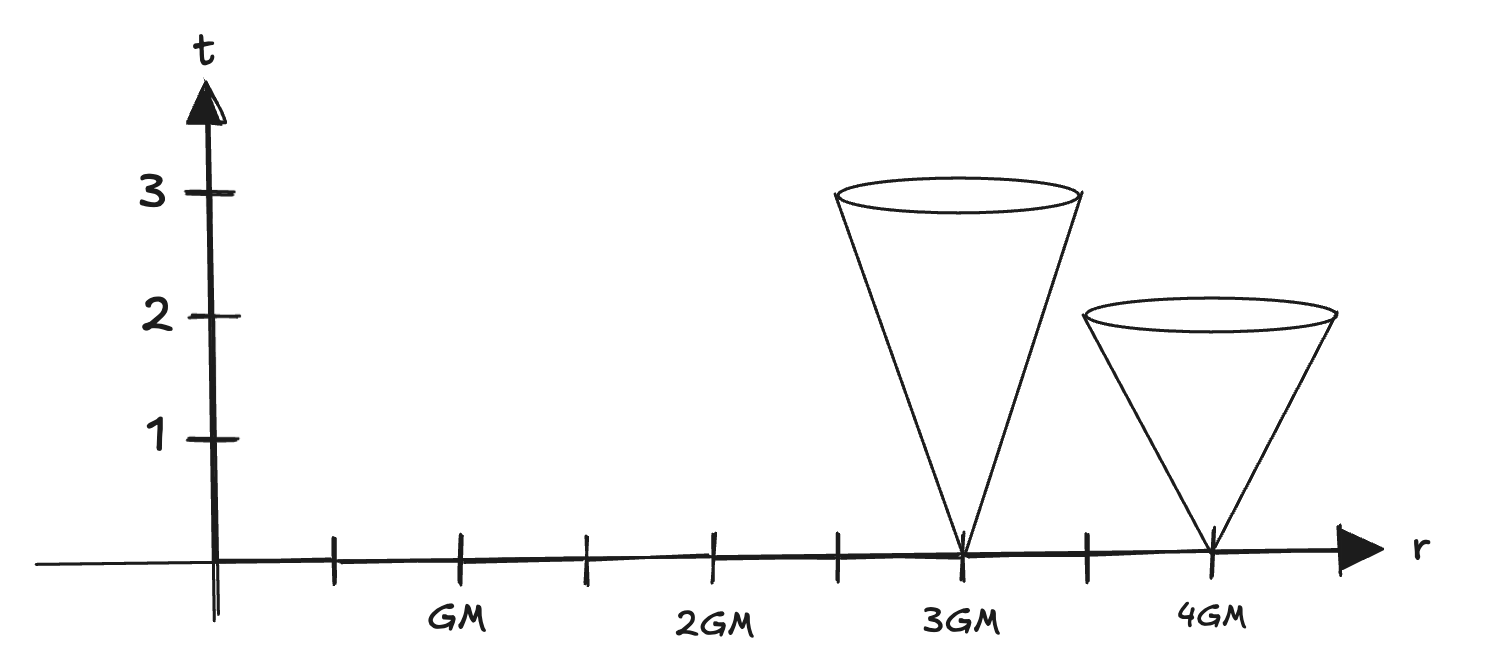
\includegraphics[scale=0.2]{ch14-p14.4-i.png}
    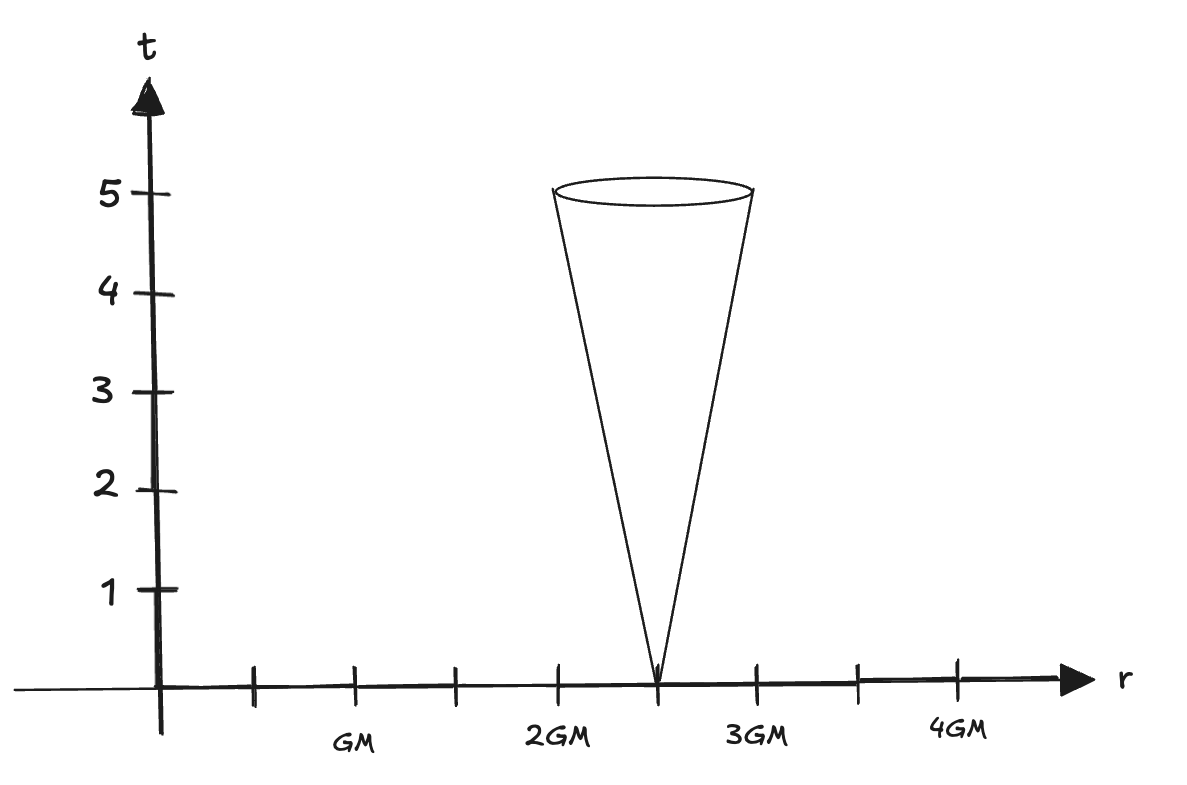
\includegraphics[scale=0.23]{ch14-p14.4-ii.png}
\end{center}
Now for $r = \frac{3}{2}GM, GM, \frac{1}{2}GM$ doing the same analysis and
considering that forward in proper time corresponds to $dr < 0$ we get that
 \begin{center}
    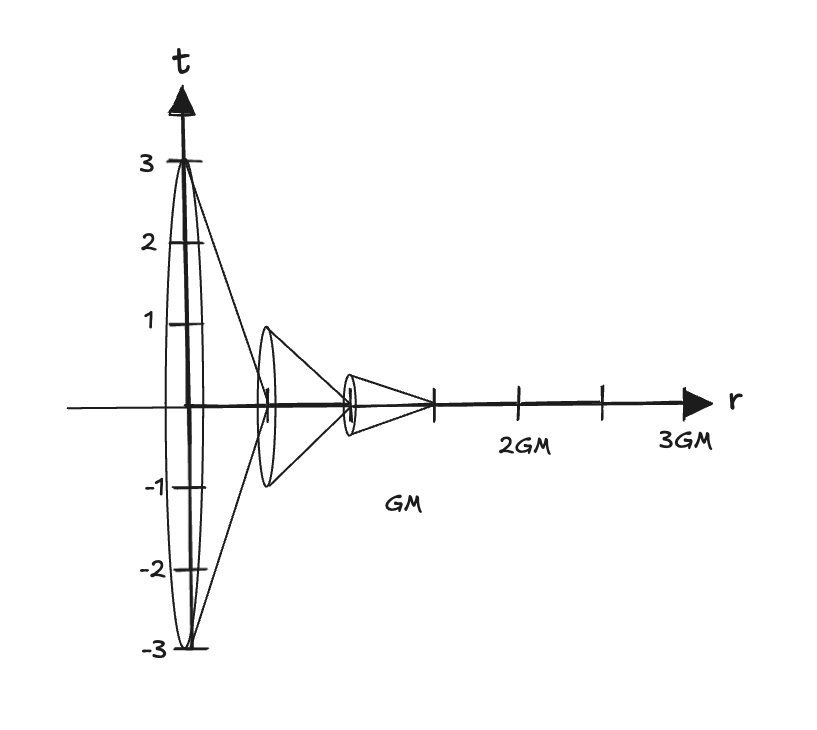
\includegraphics[scale=0.25]{ch14-p14.4-iii.png}
\end{center}
We see that the light cones in both cases narrow as they approach $r = 2GM$.
\end{proof}

\cleardoublepage
\begin{proof}{\textbf{P14.5}}
Let an observer at $R > 2GM$ launch an object with nonzero mass radially
outward with initial velocity $v_0$ as measured by the observer.
\\
Given that an object at infinity falling from rest radially has $e = 1$ then 
the same is true for an object moving radially from a radius $R$ to rest at
infinity, then from equations on Table 14.1 the particle's four velocity vector
is
\begin{align*}
    \bm{u} = \begin{bmatrix}
        \dv{t}{\tau} \\[6pt] \dv{r}{\tau} \\[6pt] 0 \\[6pt] 0
    \end{bmatrix}
    = \begin{bmatrix}
        \bigg(1 - \frac{2GM}{R}\bigg)^{-1} \\[11pt]
        \sqrt{\frac{2GM}{R}}\\[11pt] 0 \\[11pt] 0
    \end{bmatrix}
\end{align*}
Where we used that for an object travelling radially $l = 0$.
\\
On the other hand, from equation (12.10) we know that the basis vectors
of an observer at rest at $r = R$ are
\begin{align*}
    &(\bm{o}_t)^\mu = \begin{bmatrix}
        \frac{1}{\sqrt{1 - 2GM/R}}\\ 0\\ 0 \\ 0
    \end{bmatrix}
    \quad (\bm{o}_x)^\mu = \begin{bmatrix}
        0\\ 0\\ 0 \\ \frac{1}{R}
    \end{bmatrix}\\
    &(\bm{o}_y)^\mu = \begin{bmatrix}
        0\\ 0\\ -\frac{1}{R} \\ 0
    \end{bmatrix}
    \quad (\bm{o}_z)^\mu = \begin{bmatrix}
        0\\ \sqrt{1 - 2GM/R}\\ 0 \\ 0
    \end{bmatrix}
\end{align*}
Then we can compute the components of the four-velocity in the observer's frame
as $u_{obs}^t = -\bm{o}_t\cdot \bm{u}$ and $u_{obs}^\mu = \bm{o}_\mu\cdot \bm{u}$
for $\mu \in \{x, y, z\}$ hence
\begin{align*}
    u_{obs}^t &= -g_{tt}(\bm{o}_t)^t \bm{u}^t\\
    &= \bigg(1 - \frac{2GM}{R}\bigg)\bigg(1 - \frac{2GM}{R}\bigg)^{-1/2}
    \bigg(1 - \frac{2GM}{R}\bigg)^{-1}\\
    &= \frac{1}{\sqrt{1 - \frac{2GM}{R}}}\\
    \\
    u_{obs}^z &= g_{rr}(\bm{o}_z)^r \bm{u}^r\\
    &=\bigg(1 - \frac{2GM}{R}\bigg)^{-1}\sqrt{1 - \frac{2GM}{R}}
    \sqrt{\frac{2GM}{R}}\\
    &=\sqrt{\bigg(1 - \frac{2GM}{R}\bigg)^{-2}\bigg(1 - \frac{2GM}{R}\bigg)}
    \sqrt{\frac{2GM}{R}}\\
    &= \sqrt{\frac{\frac{2GM}{R}}{1 - \frac{2GM}{R}}}
\end{align*}
Also, $u_{obs}^x = u_{obs}^y = 0$ because the $\bm{u}$ components for these
velocities are 0.
\\
Then the speed of the object as measured by an observer at rest at $r = R$ is
\begin{align*}
    v_{obs} = \frac{u_{obs}^z}{u_{obs}^t} 
    &= \frac{\sqrt{\frac{\frac{2GM}{R}}{1 - \frac{2GM}{R}}}}
    {\frac{1}{\sqrt{1 - \frac{2GM}{R}}}}
    = \sqrt{\frac{2GM}{R}}
\end{align*}
But we said that the object has an initial velocity of $v_0$ as measured by
the observer then must be that
\begin{align*}
    v_0 = \sqrt{\frac{2GM}{R}}
\end{align*}
Therefore the escape speed as measured by this observer is the same as in
Newtonian mechanics.
Also, if we let $R \to 2GM$ then $v_0 = 1$ i.e. the speed of light. 
\end{proof}

\cleardoublepage
\begin{proof}{\textbf{P14.6}}
From problem P12.7 we know that basis vector $\bm{o}_t$ is
\begin{align*}
    (\bm{o}_t)^\mu = \begin{bmatrix}
        (1- 2GM/r)^{-1}\\[7pt] -\sqrt{2GM/r}\\[7pt] 0\\[7pt] 0
    \end{bmatrix}
\end{align*}
Also, from the equations 12.12a and 12.12b (the four-momentum
of a photon) we can compute $E_{obs} = - \bm{o}_t \cdot \bm{p}$ using the
metric given by equation 14.16 as follows
\begin{align*}
    E_{obs} &= - \bm{o}_t \cdot \bm{p}\\
    &= g_{tt}(\bm{o}_t)^tp^t - g_{rr}(\bm{o}_t)^rp^r\\
    &= -\bigg(\frac{2GM}{r} - 1\bigg)\bigg(1 - \frac{2GM}{r}\bigg)^{-1}
    E\bigg(1 - \frac{2GM}{r}\bigg)^{-1}\\
    &\quad+ \bigg(\frac{2GM}{r} - 1\bigg)^{-1}
    \sqrt{\frac{2GM}{r}}E\sqrt{1 - \frac{b^2}{r^2}\bigg(1 - \frac{2GM}{r}\bigg)}\\
    &= E\bigg(1 - \frac{2GM}{r}\bigg)^{-1}
    \bigg(1 - \sqrt{\frac{2GM}{r}}
    \sqrt{1 - \frac{b^2}{r^2}\bigg(1 - \frac{2GM}{r}\bigg)}\bigg)
\end{align*}
But since it's falling radially then $b = 0$ so
\begin{align*}
    E_{obs} &= E\bigg(1 - \frac{2GM}{r}\bigg)^{-1}
    \bigg(1 - \sqrt{\frac{2GM}{r}}\bigg)
\end{align*}
Finally, the fractional change in wavelength is given by
\begin{align*}
    \frac{h/\lambda_E}{h/\lambda_R}
    &= \frac{E/\sqrt{1 - \frac{2GM}{r_E}}}
    {E\bigg(1 - \frac{2GM}{r_R}\bigg)^{-1}
    \bigg(1 - \sqrt{\frac{2GM}{r_R}}\bigg)}\\
    \frac{\lambda_R}{\lambda_E}
    &= \frac{\bigg(1 - \frac{2GM}{r_R}\bigg)}
    {\sqrt{1 - \frac{2GM}{r_E}}
    \bigg(1 - \sqrt{\frac{2GM}{r_R}}\bigg)}
\end{align*}
But since $r_E = \infty$ i.e. the signal is coming from infinity
we can write that
\begin{align*}
    \frac{\lambda_R}{\lambda_E}
    &= \frac{\bigg(1 - \frac{2GM}{r_R}\bigg)}
    {\bigg(1 - \sqrt{\frac{2GM}{r_R}}\bigg)}
    = 1 + \sqrt{\frac{2GM}{r_R}}
\end{align*}
Therefore the expression is correct for $r < 2GM$ as well.
\end{proof}

\cleardoublepage
\begin{proof}{\textbf{P14.7}}
\begin{itemize}
\item [\textbf{a.}]
We want to show that curves of constant $R$ are hyperbolas so let us compute
$t^2 - r^2$, assuming $R > 1/2$ then
\begin{align*}
    t^2 - r^2 &= b^2(2R - 1)\sinh^2 T - b^2(2R - 1)\cosh^2 T\\
    &= b^2(1 - 2R)[\cosh^2 T - \sinh^2 T]\\
    &= b^2(1 - 2R)
\end{align*}
Where we used that $\cosh^2 q - \sinh^2 q = 1$ for all $q$.
\\
Therefore $t^2 - r^2 = \text{constant}$ and since $b^2(1 - 2R) < 0$ for
$R > 1/2$ then we can write that $r^2 - t^2 = |b^2(1 - 2R)|$ which implies
that the hyperbolas face rightward or leftward.

In the same way, for $R < 1/2$ we have that
\begin{align*}
    t^2 - r^2 &= b^2(1 - 2R)\cosh^2 T - b^2(1 - 2R)\sinh^2 T\\
    &= b^2(1 - 2R)[\cosh^2 T - \sinh^2 T]\\
    &= b^2(1 - 2R)
\end{align*}
But, in this case $b^2(1 - 2R) > 0$ for $R < 1/2$ so the hyperbolas face up and
down.

\item [\textbf{b.}]
We want to show that curves of constant $T$ are straight lines with constant
slope, so let us compute $t/x$ for $R > 1/2$ then
\begin{align*}
    \frac{t}{x} &= \frac{b\sqrt{2R - 1}\sinh T}{b\sqrt{2R - 1}\cosh T}
    = \frac{\sinh T}{\cosh T}
    = \frac{e^T - e^{-T}}{e^T + e^{-T}}
    = \frac{1 - e^{-2T}}{1 + e^{-2T}}
\end{align*}
We see that $0 < e^{-2T} \leq 1$ for $T \geq 0$ so the denominator is bigger
than the numerator so the slope of the line is less than 1.

In the same way, for $R < 1/2$ we have that
\begin{align*}
    \frac{t}{x} &= \frac{b\sqrt{1 - 2R}\cosh T}{b\sqrt{1 - 2R}\sinh T}
    = \frac{\cosh T}{\sinh T}
    = \frac{e^T + e^{-T}}{e^T - e^{-T}}
    = \frac{1 + e^{-2T}}{1 - e^{-2T}}
\end{align*}
Therefore in this case the slope of the line is greater than 1.

\item [\textbf{c.}]
Let the metric for this coordinate system be
\begin{align*}
    ds^2 = -(2R - 1)b^2 dT^2 + \frac{b^2 dR^2}{2R - 1} + dy^2 + dz^2
\end{align*}
We see that the coordinate $R$ is defined for $R < 1/2$ and $R > 1/2$
and there the metric is well-defined so the metric is well-defined everywhere.

\item [\textbf{d.}]
We see that the $g_{TT}$ component of the metric is negative and $g_{RR}$ is
positive when $R > 1/2$ so $R$ is a spatial coordinate and $T$ is a time
coordinate in this case.
\\
But when $R < 1/2$ we have that $g_{TT}$ is positive and $g_{RR}$ is negative
so the situation is reversed and $R$ is a time coordinate and $T$ is a spatial
coordinate. Then when $R < 1/2$ the future happens as $R \to 0$.

\item [\textbf{e.}]
Particles can cross from larger $R$s to smaller $R$s but they cannot go in
reverse because when $R < 1/2$ we know that $R$ is a time coordinate so as
soon as we cross $R = 1/2$ we cannot reverse cause that would imply going
backwards in time.
\\
We consider the line where $R = 1/2$ and $T = \infty$ to be an event horizon
in $T,R$ coordinates because the behaviour of coordinates change depending if
we are on one side or the other but this doesn't happen in $t,x$ coordinates.

\item [\textbf{f.}]
Let us consider a photon at $R = 1/2$, we know that for a photon the metric
equation looks as follows 
\begin{align*}
    0 = -(2R - 1)b^2 dT^2 + \frac{b^2 dR^2}{2R - 1} + dy^2 + dz^2
\end{align*}
Where we used that for photons $ds^2 = 0$. Then 
\begin{align*}
    \frac{b^2 dR^2}{2R - 1} &= (2R - 1)b^2 dT^2 - dy^2 - dz^2\\
    \frac{dR^2}{dT^2} &= (2R - 1)^2 - \frac{(2R - 1)}{b^2}\frac{dy^2}{dT^2}
    - \frac{(2R - 1)}{b^2}\frac{dz^2}{dT^2}
\end{align*}
So we see that when $R  = 1/2$ we get that $dR/dT = 0$ therefore the photon
must be at rest at $R = 1/2$.

On the other hand, since $ds^2 \neq 0$ for a particle of nonzero rest mass then
the particle cannot be at rest at $R = 1/2$.

\cleardoublepage
\item [\textbf{g.}]
The geodesic equation for the $T$ component is 
\begin{align*}
    \dv{\tau}(g_{T\beta}\dv{x^\beta}{\tau}) - \frac{1}{2}\partial_T
    g_{\mu\nu}\dv{x^\mu}{\tau}\dv{x^\nu}{\tau} &= 0\\
    \dv{\tau}(g_{TT}\dv{T}{\tau}) &= 0
\end{align*}
Then $g_{TT}\dv{T}{\tau}$ is equal to a constant, hence
\begin{align*}
    g_{TT}\dv{T}{\tau} &= -e\\
    -(2R - 1)b^2\dv{T}{\tau} &= -e\\
    \dv{T}{\tau} &= \frac{e}{(2R - 1)b^2}
\end{align*}
Where we named the constant $-e$.
\\
Now, let us consider the metric equation for a particle with no $y, z$ velocity,
then
\begin{align*}
    -1 &= -(2R - 1)b^2 \bigg(\dv{T}{\tau}\bigg)^2
    + \frac{b^2}{2R - 1}\bigg(\dv{R}{\tau}\bigg)^2\\
    \frac{b^2}{2R - 1}\bigg(\dv{R}{\tau}\bigg)^2
    &= (2R - 1)b^2 \bigg(\dv{T}{\tau}\bigg)^2 - 1\\
    \bigg(\dv{R}{\tau}\bigg)^2 &=
    (2R - 1)^2 \bigg(\dv{T}{\tau}\bigg)^2 - \frac{2R - 1}{b^2}\\
    \dv{R}{\tau} &= \sqrt{\frac{e^2}{b^4} - \frac{2R - 1}{b^2}}
\end{align*}
We combine this result with $dT/d\tau$ to obtain $dR/dT$ as follows
\begin{align*}
    \dv{R}{\tau}\dv{\tau}{T}
    &= \frac{(2R - 1)b^2}{e}\sqrt{\frac{e^2}{b^4} - \frac{2R - 1}{b^2}}
\end{align*}
Hence
\begin{align*}
    \dv{R}{T} &= \frac{(2R - 1)}{e}\sqrt{e^2 - b^2(2R - 1)}
\end{align*}
Let us consider now a particle released from rest at $R = 1$ and $T = 0$ then
we have that
\begin{align*}
    % 0 &= \sqrt{\frac{e^2}{b^4} - \frac{2 - 1}{b^2}}\\
    % \frac{e^2}{b^4} &= \frac{1}{b^2}\\
    % e &= b\\
    0 &= \frac{2 - 1}{e}\sqrt{e^2 - b^2(2 - 1)}\\
    e &= b
\end{align*}
So integrating $dR/dT$ we get that
\begin{align*}
    \int_0^T dT
    &= \int_1^{1/2} \frac{b}{(2R - 1)}\frac{dR}{b\sqrt{1 - (2R - 1)}}\\
    T &= \bigg[-\text{arctanh}(\sqrt{2(1 - R)})\bigg]_1^{1/2}\\
    T &= \bigg[-\text{arctanh}(\sqrt{1}) + \text{arctanh}(0)\bigg] \to \infty
\end{align*}
But integrating $dR/d\tau$ we have that
\begin{align*}
    \int_0^\tau d\tau
    &= \int_1^{1/2} \frac{dR}{b\sqrt{1 - (2R - 1)}}\\
    \tau &= \frac{1}{b}\bigg[-\sqrt{2(1 - R)}\bigg]_1^{1/2}\\
    \tau &= -\frac{1}{b}
\end{align*}
Therefore this trip requires infinite time $T$ but finite time $\tau$.
\end{itemize}
\end{proof}

\cleardoublepage
\begin{proof}{\textbf{P14.8}}
\begin{itemize}
\item [\textbf{a.}]
We know that $u = 1 - \sqrt{2GM/r}$ then
\begin{align*}
    \dv{u}{r} = \frac{1}{2r}\sqrt{\frac{2GM}{r}}
\end{align*}
From Table 14.1, we have that
\begin{align*}
    \dv{r}{t}= -\bigg(1 - \frac{2GM}{r}\bigg)
    \sqrt{1 - \frac{1}{e^2}\bigg(1 - \frac{2GM}{r}\bigg)\bigg(1 + \frac{l^2}{r^2}\bigg)}
\end{align*}
We took the negative sign because the laser is going to the blackhole.
But since the laser is falling radially from rest we have that $l = 0$ and
$e = 1$, hence
\begin{align*}
    \dv{r}{t} &= -\bigg(1 - \frac{2GM}{r}\bigg)\sqrt{\frac{2GM}{r}}
\end{align*}
Then
\begin{align*}
    \dv{r}{t}\dv{u}{r}
    &= -\bigg(1 - \frac{2GM}{r}\bigg)\sqrt{\frac{2GM}{r}}\dv{u}{r}\\
    \dv{u}{t}
    &= -\bigg(1 - \frac{2GM}{r}\bigg)\sqrt{\frac{2GM}{r}}
    \frac{1}{2r}\sqrt{\frac{2GM}{r}}\\
    \dv{u}{t}
    &= -\frac{GM}{r^2}\bigg(1 - \frac{2GM}{r}\bigg)
\end{align*}
\item [\textbf{b.}]
Using that
\begin{align*}
    1 - \frac{2GM}{r}
    = \left(1 - \sqrt{\frac{2GM}{r}}\right)\left(1 + \sqrt{\frac{2GM}{r}}\right)
\end{align*}
We can write that
\begin{align*}
    \dv{u}{t}
    &= -\frac{GM}{r^2}\left(1 - \sqrt{\frac{2GM}{r}}\right)
    \left(1 + \sqrt{\frac{2GM}{r}}\right)\\
    \dv{u}{t} &= -u\frac{GM}{r^2}\left(1 + \sqrt{\frac{2GM}{r}}\right)
\end{align*}
Then if $r \to 2GM$ we see that
\begin{align*}
    \dv{u}{t}\bigg|_{r\to 2GM} &=
    -u\frac{GM}{4(GM)^2}\left(1 + \sqrt{\frac{2GM}{2GM}}\right)
    = -\frac{u}{2GM}
\end{align*}
\item [\textbf{c.}]
The outgoing photon's energy an observer on the laser's frame measures is
\begin{align*}
    E_{obs} &= - \bm{o}_t \cdot \bm{p}\\
    &= E\bigg(1 - \frac{2GM}{r}\bigg)^{-1}
    + \bigg(1 - \frac{2GM}{r}\bigg)^{-1}\sqrt{\frac{2GM}{r}}
    E\sqrt{1 - \frac{b^2}{r^2}\bigg(1 - \frac{2GM}{r}\bigg)}\\
    &= E\bigg(1 - \frac{2GM}{r}\bigg)^{-1}
    \bigg(1 + \sqrt{\frac{2GM}{r}}
    \sqrt{1 - \frac{b^2}{r^2}\bigg(1 - \frac{2GM}{r}\bigg)}\bigg)
\end{align*}
Where we used the positive sign for $p^r$ since the photon is outgoing.
But since it's falling radially then $b = 0$ so
\begin{align*}
    E_{obs} &= E\bigg(1 - \frac{2GM}{r}\bigg)^{-1}
    \bigg(1 + \sqrt{\frac{2GM}{r}}\bigg)
\end{align*}
Finally, the fractional change in wavelength is given by
\begin{align*}
    \frac{h/\lambda_R}{h/\lambda_E}
    &= \frac{E/\sqrt{1 - \frac{2GM}{r_R}}}{E\bigg(1 - \frac{2GM}{r_E}\bigg)^{-1}
    \bigg(1 + \sqrt{\frac{2GM}{r_E}}\bigg)}\\
    \frac{\lambda_E}{\lambda_R}
    &= \frac{\bigg(1 - \frac{2GM}{r_E}\bigg)}
    {\sqrt{1 - \frac{2GM}{r_R}}\bigg(1 + \sqrt{\frac{2GM}{r_E}}\bigg)}
\end{align*}
But since $r_R \to \infty$ i.e. the signal is received at infinity
we can write that
\begin{align*}
    \frac{\lambda_R}{\lambda_E} &= \frac{\bigg(1 - \frac{2GM}{r_R}\bigg)}
    {\bigg(1 + \sqrt{\frac{2GM}{r_R}}\bigg)}
    = 1 - \sqrt{\frac{2GM}{r}}
\end{align*}
\end{itemize}
\end{proof}
\end{document}